\documentclass[
    fontsize=11pt, % Set base font size
    parskip=half,   % Add a bit of space between paragraphs
]{scrartcl} % KOMA-Script article class for a modern look

\usepackage[utf8]{inputenc}
\usepackage[T1]{fontenc}
\usepackage{xcolor}     % For defining and using colors
\usepackage{amsmath}
\usepackage{graphicx}
\usepackage{pgfplots}   % For generating plots
\pgfplotsset{compat=1.18} % Use a modern featureset for pgfplots

% --- Color Definitions ---
% Define some nice colors to use in the document.
% You can find more at: https://www.overleaf.com/learn/latex/Colors
\definecolor{primary}{HTML}{005F73}   % A nice dark teal
\definecolor{secondary}{HTML}{0A9396} % A lighter teal

% --- Font and Section Customization ---
% Redefine how sections look to use our new colors.
\addtokomafont{section}{\color{primary}\Large\bfseries}
\addtokomafont{subsection}{\color{secondary}\large\bfseries}


% --- Document Information ---
\title{\color{primary}Fourier Transforms}
\author{Matthew Lakin}



\begin{document}

\maketitle

\section{Introduction}

\section{Fourier Series}
\subsection{Definition}
A Fourier series is a way to represent a periodic function as a sum of sine and cosine functions. The general form is:
\begin{equation}
    f(x) = \frac{a_0}{2} + \sum_{n=1}^{\infty} (a_n \cos(nx) + b_n \sin(nx))
\end{equation}
where \( a_n \) and \( b_n \) are the Fourier coefficients defined as:
\begin{equation}
    a_n = \frac{2}{T} \int_0^T f(x) \cos\left(\frac{2\pi nx}{T}\right) dx
\end{equation}
\begin{equation}
    b_n = \frac{2}{T} \int_0^T f(x) \sin\left(\frac{2\pi nx}{T}\right) dx
\end{equation}

\begin{figure}[ht!]
    \centering
    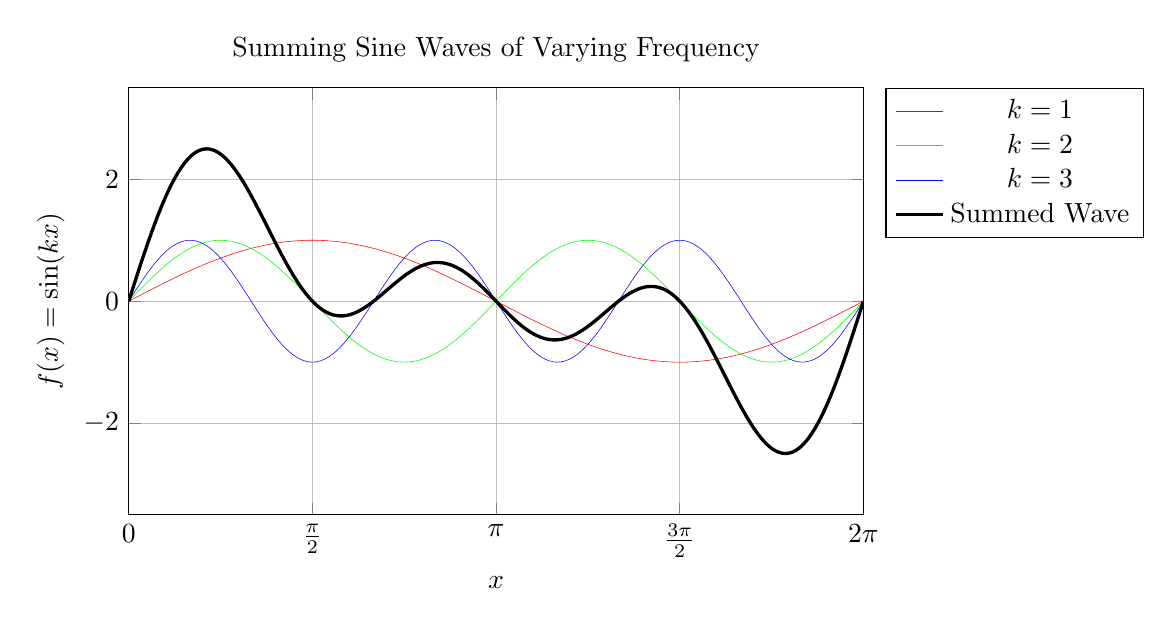
\begin{tikzpicture}
        \begin{axis}[
            height=7cm,
            width=0.9\textwidth,
            title={Summing Sine Waves of Varying Frequency},
            xlabel={$x$},
            ylabel={$f(x) = \sin(kx)$},
            legend pos=outer north east,
            grid=major,
            xmin=0, xmax={2*pi},
            ymin=-3.5, ymax=3.5,
            xtick={0, 1.5708, 3.14159, 4.71239, 6.28318},
            xticklabels={$0$, $\frac{\pi}{2}$, $\pi$, $\frac{3\pi}{2}$, $2\pi$}
        ]
        
        \addplot[domain=0:2*pi, samples=200, color=red, smooth, very thin] {sin(deg(x))};
        \addlegendentry{$k=1$}
        
        \addplot[domain=0:2*pi, samples=200, color=green, smooth, very thin] {sin(deg(2*x))};
        \addlegendentry{$k=2$}
        
        \addplot[domain=0:2*pi, samples=200, color=blue, smooth, very thin] {sin(deg(3*x))};
        \addlegendentry{$k=3$}

        \addplot[domain=0:2*pi, samples=200, color=black, smooth, very thick] {sin(deg(x)) + sin(deg(2*x)) + sin(deg(3*x))};
        \addlegendentry{Summed Wave}
        
        \end{axis}
    \end{tikzpicture}
    \label{fig:sine_waves_generated}
\end{figure}

\newpage

\section{Fourier Transforms}
\subsection{Definition}
The Fourier transform of a function \( f(x) \) is defined as
\begin{equation}
    F(s) = \int_{-\infty}^{\infty} f(x) e^{-i\frac{2\pi}{T}x} dx
\end{equation}
where \( T \) is the period of the function \( f(x) \).

\subsection{Inverse Fourier Transform}

\subsection{Discrete Fourier Transform}

\subsection{FFT.js}


\end{document}
